\documentclass{beamer}

\usepackage{Archivo}
\renewcommand{\sfdefault}{\rmdefault}
\usepackage{graphicx}
\usepackage{tikz}
\usetikzlibrary{calc}
\usepackage[most]{tcolorbox}

%% ---- Superteam Poland brand colors ----
\definecolor{stpldark}{HTML}{0B0E0F}   % near-black background
\definecolor{stplcard}{HTML}{161A1B}   % card / block surface
\definecolor{stplborder}{HTML}{1E2526}  % subtle track color for progress bar
\definecolor{stplred}{HTML}{DC143C}    % brand crimson red
\definecolor{stplwhite}{HTML}{FFFFFF}  % white
\definecolor{stplmuted}{HTML}{8A9BA8}  % muted / secondary text

\usetheme{default}
\setbeamersize{text margin left=0.85cm, text margin right=0.85cm}

%% ---- Background & base text ----
\setbeamercolor{background canvas}{bg=stpldark}
\setbeamercolor{normal text}{fg=stplwhite, bg=stpldark}
\usebeamercolor{normal text}

%% ---- Background image helpers ----
\newcommand{\stpldefaultbg}{%
  \setbeamertemplate{background}{%
    \begin{tikzpicture}[remember picture, overlay]
      \node[at=(current page.center), inner sep=0pt] {%
        
\includegraphics[width=\paperwidth,height=\paperheight]{images/bg-default.png}%
      };
      \fill[stplborder]
        (current page.north west) rectangle
        ([yshift=-2.5pt]current page.north east);
      \pgfmathsetmacro{\stplprog}{\insertframenumber/\inserttotalframenumber}
      \fill[stplred]
        (current page.north west) rectangle
        ($(current page.north west)+(\stplprog\paperwidth,-2.5pt)$);
    \end{tikzpicture}%
  }%
}
\newcommand{\stplherobg}{%
  \setbeamertemplate{background}{%
    
\includegraphics[width=\paperwidth,height=\paperheight]{images/bg-hero.png}%
  }%
}
\stpldefaultbg

%% ---- Structure ----
\setbeamercolor{structure}{fg=stplred}

%% ---- Title slide metadata ----
\setbeamercolor{title}{fg=stplwhite}
\setbeamercolor{subtitle}{fg=stplred}
\setbeamercolor{author}{fg=stplwhite}
\setbeamercolor{institute}{fg=stplmuted}
\setbeamercolor{date}{fg=stplmuted}

%% ---- Frame title: flat, no box background ----
\setbeamercolor{frametitle}{fg=stplwhite, bg=}
\setbeamerfont{frametitle}{size=\large, series=\bfseries}
\setbeamertemplate{frametitle}{%
  \vspace{0.35cm}%
  {\centering\insertframetitle\par}%
  \nointerlineskip\vspace{0.18cm}%
  \hfil{\color{stplred}\rule{2.2cm}{1.5pt}}\hfil\par%
}



%% ---- Incremental reveals ----
\beamerdefaultoverlayspecification{<+->}

%% ---- Bullet items ----
\setbeamercolor{itemize item}{fg=stplred}
\setbeamercolor{itemize subitem}{fg=stplmuted}
\setbeamercolor{itemize subsubitem}{fg=stplmuted}
\setbeamertemplate{itemize item}{\bfseries\textendash}
\setbeamertemplate{itemize subitem}{\small\textendash}
\setbeamercolor{enumerate item}{fg=stplred}
\setbeamercolor{enumerate subitem}{fg=stplmuted}

%% ---- Blocks (flat left-accent via tcolorbox) ----
\tcbset{
  stplbase/.style={
    enhanced, breakable,
    colback=stplcard, coltext=stplwhite,
    coltitle=stplwhite, fonttitle=\bfseries,
    boxrule=0pt, leftrule=3pt,
    arc=0pt, outer arc=0pt,
    top=5pt, bottom=5pt, left=7pt, right=7pt,
    toptitle=4pt, bottomtitle=4pt,
    titlerule=0pt,
  },
}
\renewenvironment{block}[1]{%
  \begin{tcolorbox}[stplbase, colframe=stplred, title={#1}]%
}{%
  \end{tcolorbox}%
}
\renewenvironment{alertblock}[1]{%
  \begin{tcolorbox}[stplbase, colframe=stplred!75!black,
    colback=stplred!10!stplcard, title={#1}]%
}{%
  \end{tcolorbox}%
}
\renewenvironment{exampleblock}[1]{%
  \begin{tcolorbox}[stplbase, colframe=stplmuted, title={#1}]%
}{%
  \end{tcolorbox}%
}

%% ---- Table of contents ----
\setbeamercolor{section in toc}{fg=stplwhite}
\setbeamercolor{subsection in toc}{fg=stplmuted}
\setbeamertemplate{section in toc}{%
  {\color{stplred}\textbf{\textendash}}\hspace{0.5em}\inserttocsection%
}

%% ---- Footline: minimal ----
\setbeamertemplate{footline}{%
  \begin{beamercolorbox}[wd=\paperwidth, ht=0pt, dp=0.55cm]{normal text}%
    \hspace{0.85cm}%
    
\includegraphics[height=1.6ex]{images/stpl-logo.png}%
    \hfill%
    \textcolor{stplmuted}{\tiny\insertframenumber\,/\,\inserttotalframenumber}%
    \hspace{0.85cm}%
  \end{beamercolorbox}%
}
\setbeamertemplate{navigation symbols}{}

%% ---- Title frame helper (uses hero background) ----
\newcommand{\maketitleframe}{%
  \stplherobg
  \begin{frame}[plain]%
    \titlepage%
  \end{frame}%
  \stpldefaultbg
}

%% ---- Section divider slides ----
\AtBeginSection[]{%
  \stplherobg
  \begin{frame}[plain]
    \begin{tikzpicture}[remember picture, overlay]
      \fill[stplred, opacity=0.07]
        ([xshift=-2.5cm]current page.east) circle (5.5cm);
      \fill[stplred]
        (current page.north west) rectangle ([xshift=5pt]current page.south west);
    \end{tikzpicture}%
    \vfill
    \hspace{0.1\paperwidth}%
    \begin{minipage}{0.8\paperwidth}
      \textcolor{stplmuted}{\small Section \thesection}\\[0.35cm]
      {\color{stplwhite}\LARGE\bfseries\insertsectionhead}\\[0.25cm]
      {\color{stplred}\rule{3cm}{1.5pt}}
    \end{minipage}%
    \vfill
  \end{frame}%
  \stpldefaultbg
}

%% ---- Title page ----
\setbeamertemplate{title page}{%
  \begin{tikzpicture}[remember picture, overlay]
    \fill[stplred]
      (current page.north west) rectangle ([xshift=5pt]current page.south west);
    \fill[stplred, opacity=0.07]
      ([xshift=-3cm,yshift=3cm]current page.north east) circle (5.5cm);
    \fill[stplred, opacity=0.04]
      ([yshift=-1.5cm]current page.south east) circle (3.5cm);
  \end{tikzpicture}%
  \vfill
  \hspace{0.08\paperwidth}%
  \begin{minipage}{0.85\paperwidth}
    
\includegraphics[width=3cm]{images/stpl-logo.png}\par
    \vspace{0.8cm}
    {\usebeamerfont{title}\usebeamercolor[fg]{title}\inserttitle}\par
    \vspace{0.2cm}
    {\color{stplred}\rule{3cm}{1.5pt}}\par
    \vspace{0.3cm}
    {\usebeamerfont{subtitle}\usebeamercolor[fg]{subtitle}\insertsubtitle}\par
    \vspace{0.65cm}
    {\usebeamerfont{author}\usebeamercolor[fg]{author}\insertauthor}\par
    \vspace{0.12cm}
    {\small\textcolor{stplmuted}{\insertinstitute\enspace·\enspace\insertdate}}
  \end{minipage}%
  \vfill
}


\usepackage[utf8]{inputenc}
\usepackage[T1]{fontenc}
\usetikzlibrary{positioning, arrows.meta}

\title{Paradygmat Web3}
\subtitle{Solana Bootcamp --- dla dewelopera Web2}
\author{}
\institute{Superteam Poland}

\begin{document}

\maketitleframe

\begin{frame}{Plan}
  \tableofcontents
\end{frame}

% ================================================================
\section{Web2 vs Web3}

% TODO: 1. Z wizji do warsztatu --- transition (no helper block)
\begin{frame}{Z wizji do warsztatu}
  \begin{itemize}
    \item Lekcja 0 pokazała, \textbf{czemu} blockchain w ogóle istnieje
    \item Teraz: \textbf{jak} to działa od strony dewelopera
    \item Punkt wyjścia --- co znika z Web2 stacku?
  \end{itemize}
\end{frame}

% TODO: 2. Web2 w jednym zdaniu --- problem hook (alertblock: jeden właściciel prawdy)
\begin{frame}{Web2 w jednym zdaniu}
  \begin{itemize}
    \item Klient pyta \textbf{centralny serwer}, który ufa sam sobie
    \item Baza danych \textbf{pod kontrolą dostawcy} --- prywatna
    \item Aplikacja działa, dopóki działa operator
  \end{itemize}
  \vspace{0.2cm}
  \begin{center}
    \begin{tikzpicture}[
        every node/.style={font=\scriptsize\bfseries},
        box/.style={
          draw=stplred, line width=1pt,
          fill=stplcard, text=stplwhite,
          rounded corners=2pt,
          minimum width=1.7cm, minimum height=0.6cm,
          align=center,
        },
        dbbox/.style={
          draw=stplred, line width=1pt,
          fill=stplred, text=stplwhite,
          rounded corners=2pt,
          minimum width=1.7cm, minimum height=0.6cm,
          align=center,
        },
        arr/.style={-latex, draw=stplred, line width=1pt},
        lbl/.style={font=\tiny\itshape, text=stplmuted},
      ]
      % Stage 1: Klient + Serwer + HTTPS arrow
      \node[box] (cli) {Klient};
      \node[box, right=1.4cm of cli] (srv) {Serwer firmy};
      \node[dbbox, right=1.4cm of srv, visible on=<2->] (db) {Prywatna DB};
      \draw[arr] (cli) -- node[lbl, above]{HTTPS} (srv);

      % Stage 2: Prywatna DB + zaufanie arrow
      \begin{scope}[visible on=<2->]
        \draw[arr] (srv) -- node[lbl, above]{zaufanie} (db);
      \end{scope}
    \end{tikzpicture}
  \end{center}
  \begin{alertblock}{Jeden właściciel prawdy}
    Firma decyduje, co jest w bazie. Trzeba jej zaufać, że nie kłamie.
  \end{alertblock}
\end{frame}

% TODO: 3. Web3 w jednym zdaniu --- mechanism (exampleblock: backend staje się programem)
\begin{frame}{Web3 w jednym zdaniu}
  \begin{itemize}
    \item Klient wysyła \textbf{podpisaną transakcję} do sieci
    \item Logika żyje on-chain jako \textbf{program}
    \item Dane w koncie blockchain --- \textbf{bezaufaniowe wykonanie}
  \end{itemize}
  \vspace{0.2cm}
  \begin{center}
    \begin{tikzpicture}[
        every node/.style={font=\scriptsize\bfseries},
        box/.style={
          draw=stplred, line width=1pt,
          fill=stplcard, text=stplwhite,
          rounded corners=2pt,
          minimum width=1.7cm, minimum height=0.6cm,
          align=center,
        },
        accbox/.style={
          draw=stplred, line width=1pt,
          fill=stplred, text=stplwhite,
          rounded corners=2pt,
          minimum width=1.7cm, minimum height=0.6cm,
          align=center,
        },
        arr/.style={-latex, draw=stplred, line width=1pt},
        lbl/.style={font=\tiny\itshape, text=stplmuted},
      ]
      % Stage 1: Klient
      \node[box] (cli) {Klient};
      \node[draw=stplred, line width=1pt, fill=stplcard,
            rounded corners=2pt,
            minimum width=2.0cm, minimum height=1.0cm,
            right=1.4cm of cli, visible on=<2->] (cluster) {};
      \node[accbox, right=1.4cm of cluster, visible on=<3->] (acc) {Konta};

      % Stage 2: Klaster (3-dot cluster) + podpis arrow
      \begin{scope}[visible on=<2->]
        \node[lbl] at ($(cluster.north)+(0,-0.2cm)$) {Klaster};
        \node[circle, fill=stplred, inner sep=1.5pt] at ($(cluster.center)+(-0.45,-0.08)$) {};
        \node[circle, fill=stplred, inner sep=1.5pt] at ($(cluster.center)+(0,-0.08)$) {};
        \node[circle, fill=stplred, inner sep=1.5pt] at ($(cluster.center)+(0.45,-0.08)$) {};
        \draw[arr] (cli) -- node[lbl, above]{podpis} (cluster);
      \end{scope}

      % Stage 3: Konta + stan arrow
      \begin{scope}[visible on=<3->]
        \draw[arr] (cluster) -- node[lbl, above]{stan} (acc);
      \end{scope}
    \end{tikzpicture}
  \end{center}
  \begin{exampleblock}{Backend staje się programem}
    Nie ma serwera firmy --- jest klaster węzłów, który każdy może odpytać.
  \end{exampleblock}
\end{frame}

% TODO: 4. RPC node --- term debut (block; analogia: bankomat dowolnej sieci)
\begin{frame}{RPC node}
  \begin{columns}[T]
    \column{0.50\textwidth}
      \begin{itemize}
        \item Frontend potrzebuje \textbf{okna na łańcuch}
        \item Setki publicznych węzłów, to samo API
        \item Analogia --- \textbf{bankomat dowolnej sieci}
        \item \textbf{Remote Procedure Call (RPC)}
      \end{itemize}
    \column{0.48\textwidth}
      \begin{center}
        \begin{tikzpicture}[
            every node/.style={font=\scriptsize\bfseries},
            box/.style={
              draw=stplred, line width=0.8pt,
              fill=stplcard, text=stplwhite,
              rounded corners=2pt,
              minimum width=1.3cm, minimum height=0.5cm,
              align=center,
            },
            clbox/.style={
              draw=stplred, line width=0.8pt,
              fill=stplred, text=stplwhite,
              rounded corners=2pt,
              minimum width=1.3cm, minimum height=0.5cm,
              align=center,
            },
            arr/.style={-latex, draw=stplred, line width=0.7pt},
          ]
          % Stage 1: Frontend
          \node[box] (fe) at (0,0) {Frontend};
          \node[box, visible on=<2->] (r1) at (1.8, 0.8) {Helius};
          \node[box, visible on=<2->] (r2) at (1.8, 0) {QuickNode};
          \node[box, visible on=<2->] (r3) at (1.8,-0.8) {własny};
          \node[clbox, visible on=<3->] (cl) at (3.6, 0) {Klaster};

          % Stage 2: RPC fan from Frontend
          \begin{scope}[visible on=<2->]
            \draw[arr] (fe) -- (r1);
            \draw[arr] (fe) -- (r2);
            \draw[arr] (fe) -- (r3);
          \end{scope}

          % Stage 3: arrows into Klaster
          \begin{scope}[visible on=<3->]
            \draw[arr] (r1) -- (cl);
            \draw[arr] (r2) -- (cl);
            \draw[arr] (r3) -- (cl);
          \end{scope}
        \end{tikzpicture}
      \end{center}
  \end{columns}
  \vspace{0.3cm}
  \begin{block}{Definicja}
    \textbf{RPC node} --- węzeł sieci, który przyjmuje zapytania klienta
    i zwraca aktualny stan lub przekazuje transakcję do klastra.
  \end{block}
\end{frame}

% ================================================================
\section{Co się zmienia}

% TODO: 5. Read vs Write --- A-vs-B opposition (no helper block)
%       Sequential reveal: Read (overlays 1-4), then Write (overlays 7-10).
\begin{frame}{Read vs Write}
  % Both columns open with a block, and each block self-reveals with \pause
  % (see preamble). On a block-first frame those leading pauses push the first
  % bullet to overlay 4, leaving three blank opening slides. Pull the pause
  % counter back so Read's first bullet lands on overlay 1 instead.
  \addtocounter{beamerpauses}{-3}%
  \begin{columns}
    \column{0.48\textwidth}
      \begin{block}{Read}
        \centering
        \begin{tikzpicture}[
            every node/.style={font=\tiny\bfseries},
            b/.style={
              draw=stplred, line width=0.7pt,
              fill=stplcard, text=stplwhite,
              rounded corners=2pt,
              minimum width=0.9cm, minimum height=0.4cm, align=center,
            },
            arr/.style={-latex, draw=stplred, line width=0.7pt},
          ]
          % Stage 1 (<1->): request out
          \node[b] (c) {Klient};
          \node[b, right=0.6cm of c] (r) {RPC};
          \draw[arr] ([yshift=2.5pt]c.east) -- ([yshift=2.5pt]r.west);
          % Stage 2 (<3->): response back, paired with "Odpowiedź natychmiast"
          \begin{scope}[visible on=<3->]
            \draw[arr] ([yshift=-2.5pt]r.west) -- ([yshift=-2.5pt]c.east);
          \end{scope}
        \end{tikzpicture}
        \vspace{0.1cm}
        \begin{itemize}
          \item<+-> Gratis, bez podpisu
          \item<+-> Dowolny węzeł RPC
          \item<+-> Odpowiedź natychmiast
          \item<+-> Np. podgląd salda konta
        \end{itemize}
      \end{block}

    \column{0.48\textwidth}
      \begin{alertblock}{Write}
        \centering
        \begin{tikzpicture}[
            every node/.style={font=\tiny\bfseries},
            b/.style={
              draw=stplred, line width=0.7pt,
              fill=stplcard, text=stplwhite,
              rounded corners=2pt,
              minimum width=0.7cm, minimum height=0.4cm, align=center,
            },
            bk/.style={
              draw=stplred, line width=0.7pt,
              fill=stplred, text=stplwhite,
              rounded corners=2pt,
              minimum width=0.5cm, minimum height=0.4cm, align=center,
            },
            arr/.style={-latex, draw=stplred, line width=0.7pt},
          ]
          % Layout reserved from the start; nodes appear with their Write
          % bullets (Transakcja <7->, Opłata <8->, Czeka <9->).
          \node[b, visible on=<7->] (c) {Klient};
          \node[b, right=0.2cm of c, visible on=<7->] (r) {RPC};
          \node[b, right=0.2cm of r, visible on=<8->] (k) {Klaster};
          \node[bk, right=0.2cm of k, visible on=<9->] (ok) {ack};
          % Klient → RPC (with "Transakcja")
          \begin{scope}[visible on=<7->]
            \draw[arr] (c) -- (r);
          \end{scope}
          % → Klaster (with "Opłata")
          \begin{scope}[visible on=<8->]
            \draw[arr] (r) -- (k);
          \end{scope}
          % → ack (with "Czeka")
          \begin{scope}[visible on=<9->]
            \draw[arr] (k) -- (ok);
          \end{scope}
        \end{tikzpicture}
        \vspace{0.1cm}
        \begin{itemize}
          \item<+-> \textbf{Transakcja} podpisana kluczem
          \item<+-> Opłata sieciowa za włączenie
          \item<+-> Czeka na potwierdzenie klastra
          \item<+-> Np. wysłanie tokena
        \end{itemize}
      \end{alertblock}
  \end{columns}
\end{frame}

% TODO: 6. Bezserwerowa architektura --- benefit + ryzyko (alertblock: kod publiczny i niezmienny)
\begin{frame}{Bezserwerowa architektura}
  \begin{columns}[T]
    \column{0.56\textwidth}
      \begin{itemize}
        \item Kod nie żyje na \textbf{twoim} serwerze
        \item Brak uptime'u, deploymentu, VPS
        \item Stan \textbf{publiczny on-chain}
        \item Dev pisze logikę, nie infrastrukturę
      \end{itemize}
    \column{0.42\textwidth}
      \begin{center}
        \begin{tikzpicture}[
            every node/.style={font=\tiny\bfseries, align=center},
            vbox/.style={
              draw=stplmuted, line width=0.6pt,
              fill=stplcard, text=stplwhite,
              rounded corners=2pt,
              minimum width=1.3cm, minimum height=0.9cm,
            },
            lnk/.style={draw=stplmuted, line width=0.5pt},
            lbl/.style={font=\tiny\itshape, text=stplmuted},
          ]
          % Stage 1: one validator, with the program inside
          \node[vbox] (v1) at (0,0.55)    {Walidator\\\textcolor{stplred}{Program}};
          % Stage 2: same program replicated on every node + interconnections
          \begin{scope}[visible on=<2->]
            \node[vbox] (v2) at (1.6,0.55)  {Walidator\\\textcolor{stplred}{Program}};
            \node[vbox] (v3) at (3.2,0.55)  {Walidator\\\textcolor{stplred}{Program}};
            \node[vbox] (v4) at (0,-0.65)   {Walidator\\\textcolor{stplred}{Program}};
            \node[vbox] (v5) at (1.6,-0.65) {Walidator\\\textcolor{stplred}{Program}};
            \node[vbox] (v6) at (3.2,-0.65) {Walidator\\\textcolor{stplred}{Program}};
            % Adjacency: top + bottom rows, three verticals
            \draw[lnk] (v1) -- (v2);
            \draw[lnk] (v2) -- (v3);
            \draw[lnk] (v4) -- (v5);
            \draw[lnk] (v5) -- (v6);
            \draw[lnk] (v1) -- (v4);
            \draw[lnk] (v2) -- (v5);
            \draw[lnk] (v3) -- (v6);
            % Diagonals to v5 (routes through empty space between boxes)
            \draw[lnk] (v1) -- (v5);
            \draw[lnk] (v3) -- (v5);
            \node[lbl] at (1.6,-1.35) {ten sam kod na każdym węźle};
          \end{scope}
        \end{tikzpicture}
      \end{center}
  \end{columns}
  \vspace{0.1cm}
  \begin{alertblock}{Druga strona medalu}
    Kod publiczny i niezmienny --- błąd też publiczny i trudny do cofnięcia.
  \end{alertblock}
\end{frame}

% TODO: 7. Portfel jako tożsamość --- soft debut kluczy (exampleblock: podpis odręczny)
%       Asymmetric crypto deep-dive lives in L6; here keep it intuitive.
\begin{frame}{Portfel jako tożsamość}
  \begin{itemize}
    \item Brak hasła --- jest \textbf{para kluczy}
    \item \textbf{Klucz prywatny} podpisuje transakcję
    \item \textbf{Klucz publiczny} weryfikuje podpis i jest adresem
    \item Portfel trzyma klucze i podpisuje w imieniu użytkownika
  \end{itemize}
  \vspace{0.25cm}
  \begin{center}
    \begin{tikzpicture}[
        every node/.style={font=\scriptsize\bfseries, align=center},
        box/.style={
          draw=stplred, line width=1pt,
          fill=stplcard, text=stplwhite,
          rounded corners=2pt,
          minimum width=2.0cm, minimum height=0.7cm,
        },
        outbox/.style={
          draw=stplred, line width=1pt,
          fill=stplred, text=stplwhite,
          rounded corners=2pt,
          minimum width=2.0cm, minimum height=0.7cm,
        },
        arr/.style={-latex, draw=stplred, line width=1pt},
        lbl/.style={font=\tiny\itshape, text=stplmuted},
      ]
      % Stage 1: niepodpisana Transakcja --- input
      \node[box] (tx) at (0, 0) {Transakcja};
      % Stage 2: Klucz prywatny podpisuje --- produkuje Podpisaną transakcję
      \node[box, visible on=<2->] (priv) at (3.7, 1.3) {Klucz\\prywatny};
      \node[outbox, visible on=<2->] (sig) at (3.7, 0) {Podpisana\\transakcja};
      % Stage 3: Klucz publiczny weryfikuje --- produkuje wynik
      \node[box, visible on=<3->] (pub) at (7.4, 1.3) {Klucz\\publiczny};
      \node[outbox, visible on=<3->] (ver) at (7.4, 0) {Weryfikacja\,$\checkmark$};

      \begin{scope}[visible on=<2->]
        \draw[arr] (tx)   -- (sig);
        \draw[arr] (priv) -- node[lbl, right]{podpisuje} (sig);
      \end{scope}
      \begin{scope}[visible on=<3->]
        \draw[arr] (sig)  -- (ver);
        \draw[arr] (pub)  -- node[lbl, right]{weryfikuje} (ver);
      \end{scope}
    \end{tikzpicture}
  \end{center}
  \vspace{0.1cm}
  \begin{exampleblock}{Analogia}
    Podpis odręczny nie do podrobienia --- ale i bez opcji resetu.
  \end{exampleblock}
\end{frame}

% TODO: 8. Konsekwencje UX --- (alertblock: utrata klucza = utrata dostępu)
\begin{frame}{Konsekwencje UX}
  \begin{itemize}
    \item Brak ekranu \textit{,,zapomniałem hasła''} --- nie ma kto resetować
    \item Tożsamość \textbf{przenośna} --- jeden portfel = login do tysięcy aplikacji
    \item User jest \textbf{właścicielem} swojej tożsamości, nie operator
    \item Onboarding krótszy --- bez formularzy i maili weryfikacyjnych
  \end{itemize}
  \vspace{0.3cm}
  \begin{alertblock}{Cena suwerenności}
    Utrata klucza = utrata dostępu --- projektujemy świadomie
    (seed phrase, portfele sprzętowe).
  \end{alertblock}
\end{frame}

% TODO: 9. Mapa stacku --- single TikZ visual: Frontend / Wallet Adapter / RPC / Klaster / Program / Konta
%       Override <+-> for this slide --- it lands all at once.
\begin{frame}<1>{Mapa stacku Web3}
  \vspace{0.2cm}
  \begin{center}
    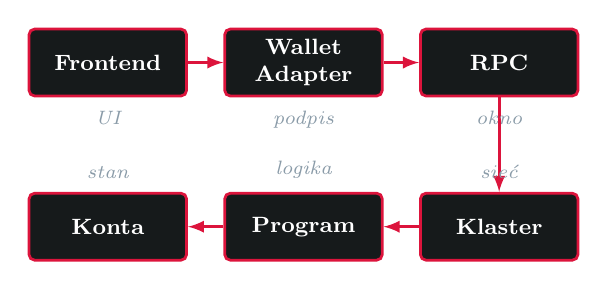
\begin{tikzpicture}[
        node distance=0.45cm,
        every node/.style={font=\footnotesize\bfseries},
        box/.style={
          draw=stplred, line width=1pt,
          fill=stplcard, text=stplwhite,
          rounded corners=2pt,
          minimum width=2.0cm, minimum height=0.85cm,
          align=center,
        },
        chain/.style={
          -latex, draw=stplred, line width=1pt,
        },
        label/.style={
          font=\scriptsize\itshape, text=stplmuted,
        },
      ]
      \node[box] (fe) {Frontend};
      \node[box, right=of fe] (wa) {Wallet\\Adapter};
      \node[box, right=of wa] (rpc) {RPC};
      \node[box, below=1.2cm of rpc] (cluster) {Klaster};
      \node[box, left=of cluster] (prog) {Program};
      \node[box, left=of prog] (acc) {Konta};

      \draw[chain] (fe) -- (wa);
      \draw[chain] (wa) -- (rpc);
      \draw[chain] (rpc) -- (cluster);
      \draw[chain] (cluster) -- (prog);
      \draw[chain] (prog) -- (acc);

      \node[label, below=0.05cm of fe] {UI};
      \node[label, below=0.05cm of wa] {podpis};
      \node[label, below=0.05cm of rpc] {okno};
      \node[label, above=0.05cm of cluster] {sieć};
      \node[label, above=0.05cm of prog] {logika};
      \node[label, above=0.05cm of acc] {stan};
    \end{tikzpicture}
  \end{center}
  \vspace{0.2cm}
  \begin{center}
    \textcolor{stplmuted}{\small Klient $\rightarrow$ podpis $\rightarrow$ RPC $\rightarrow$ klaster $\rightarrow$ program $\rightarrow$ konta}
  \end{center}
\end{frame}

\begin{frame}<1>{Mapa stacku Web3}
  \vspace{0.2cm}
  \begin{center}
    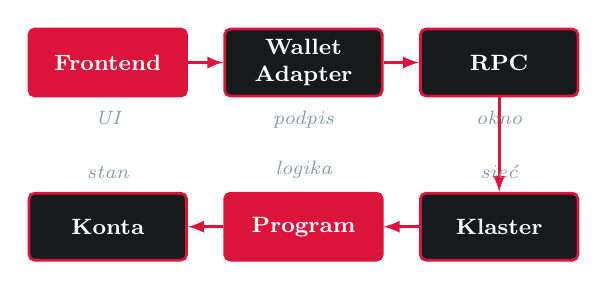
\begin{tikzpicture}[
        node distance=0.45cm,
        every node/.style={font=\footnotesize\bfseries},
        box/.style={
          draw=stplred, line width=1pt,
          fill=stplcard, text=stplwhite,
          rounded corners=2pt,
          minimum width=2.0cm, minimum height=0.85cm,
          align=center,
        },
        devbox/.style={
          draw=stplred, line width=1pt,
          fill=stplred, text=stplwhite,
          rounded corners=2pt,
          minimum width=2.0cm, minimum height=0.85cm,
          align=center,
        },
        chain/.style={
          -latex, draw=stplred, line width=1pt,
        },
        label/.style={
          font=\scriptsize\itshape, text=stplmuted,
        },
      ]
      \node[devbox] (fe) {Frontend};
      \node[box, right=of fe] (wa) {Wallet\\Adapter};
      \node[box, right=of wa] (rpc) {RPC};
      \node[box, below=1.2cm of rpc] (cluster) {Klaster};
      \node[devbox, left=of cluster] (prog) {Program};
      \node[box, left=of prog] (acc) {Konta};

      \draw[chain] (fe) -- (wa);
      \draw[chain] (wa) -- (rpc);
      \draw[chain] (rpc) -- (cluster);
      \draw[chain] (cluster) -- (prog);
      \draw[chain] (prog) -- (acc);

      \node[label, below=0.05cm of fe] {UI};
      \node[label, below=0.05cm of wa] {podpis};
      \node[label, below=0.05cm of rpc] {okno};
      \node[label, above=0.05cm of cluster] {sieć};
      \node[label, above=0.05cm of prog] {logika};
      \node[label, above=0.05cm of acc] {stan};
    \end{tikzpicture}
  \end{center}
  \vspace{0.2cm}
  \begin{center}
    \textcolor{stplred}{\small\bfseries Dev pisze Frontend i Program} ---
    \textcolor{stplmuted}{\small reszta stacku jest gotowa}
  \end{center}
\end{frame}

% ================================================================
\section{Podsumowanie}

% TODO: 10. Podsumowanie --- recap czterech różnic (Web3 vs Web2)
\begin{frame}{Podsumowanie}
  \begin{itemize}
    \item<1-> \textbf{Portfel} zamiast serwera tożsamości
    \item<2-> \textbf{RPC} zamiast prywatnego API
    \item<3-> Stan \textbf{publiczny on-chain}, nie w bazie
    \item<4-> Read gratis, write z podpisem i opłatą
  \end{itemize}
  \vspace{0.2cm}
  \begin{center}
    \begin{tikzpicture}[
        every node/.style={font=\scriptsize\bfseries},
        b/.style={
          draw=stplred, line width=0.8pt,
          fill=stplcard, text=stplwhite,
          rounded corners=2pt,
          minimum width=1.8cm, minimum height=0.5cm, align=center,
        },
        r/.style={
          draw=stplred, line width=0.8pt,
          fill=stplred, text=stplwhite,
          rounded corners=2pt,
          minimum width=1.8cm, minimum height=0.5cm, align=center,
        },
        arr/.style={-latex, draw=stplred, line width=0.7pt},
        lbl/.style={font=\tiny\itshape, text=stplmuted},
      ]
      % Headers (always)
      \node[lbl] at (0, 1.95)   {Web2};
      \node[lbl] at (3.0, 1.95) {Web3};
      % Stage 1: login row
      \node[b] (w2c) at (0, 1.4)   {Klient};
      \node[b] (w3c) at (3.0, 1.4) {Portfel};
      % Stage 2: API row
      \node[b, visible on=<2->] (w2s) at (0, 0.7)   {Serwer};
      \node[b, visible on=<2->] (w3r) at (3.0, 0.7) {RPC};
      \begin{scope}[visible on=<2->]
        \draw[arr] (w2c) -- (w2s);
        \draw[arr] (w3c) -- (w3r);
      \end{scope}
      % Stage 3: state row
      \node[r, visible on=<3->] (w2d) at (0, 0)   {Prywatna DB};
      \node[r, visible on=<3->] (w3a) at (3.0, 0) {On-chain};
      \begin{scope}[visible on=<3->]
        \draw[arr] (w2s) -- (w2d);
        \draw[arr] (w3r) -- (w3a);
      \end{scope}
    \end{tikzpicture}
  \end{center}
  \vspace{0.2cm}
  \begin{center}
    \uncover<5->{\textcolor{stplmuted}{Wiesz \textbf{JAK} pracuje Web3 dev.
    Od kolejnej lekcji --- co się na tym modelu buduje: DeFi.}}
  \end{center}
\end{frame}

% ================================================================
\begin{frame}[plain]
  \begin{center}
    \vfill
    {\Huge\bfseries\color{stplwhite} gn}
    \vfill
  \end{center}
\end{frame}

\end{document}
